\documentclass{article}
\usepackage[utf8]{inputenc}
\usepackage{geometry}
\usepackage{graphicx}
\usepackage{pgfplots}
\usepackage{amsmath}
\usepackage{amssymb}
\usepackage{amsfonts}
\usepackage[thmmarks, amsmath, thref]{ntheorem}
\usepackage{mdframed}
\usepackage{amsthm}
\usepackage{physics}
\usepackage{proof}
\usepackage{derivative}
\usepackage{hyperref}
\usepackage{wrapfig}
\usepackage{amsthm}
\usepackage{xcolor}
\renewcommand{\theenumi}{\roman{enumi}}

\theoremstyle{nonumberplain}
\theoremheaderfont{\itshape}
\theorembodyfont{\upshape}
\theoremseparator{.}
\theoremsymbol{\ensuremath{\square}}
\theoremsymbol{\ensuremath{\blacksquare}}
\newtheorem{solution}{Solution}
\theoremseparator{. ---}
\theoremsymbol{\mbox{\texttt{;o)}}}

\pgfplotsset{compat=1.18}
\begin{document}
\hspace{12cm}$\mathfrak{Andres \,\, Lopez \,\, Gonzalez}$\\\\
1. Construye la superficie de Riemann \( \mathfrak{S}_{f} \) de la función \( f(z)=\sqrt[n]{z} \), para cada \( n \in \mathbb{N} \). ¿Si \( f(z)=\sqrt[n]{z} \) y \( g(z)=\sqrt[m]{z} \) con \( n, m \in \mathbb{N} \) y \( m \neq n \), cambia en algo la topología de \( \mathfrak{S}_{f} \) y \( \mathfrak{S}_{g} \) ? ¿En qué podrías decir que son distintas \( \mathfrak{S}_{f} \) y \( \mathfrak{S}_{g} ? \) \\

\textbf{*Ver al final del documento una pequeña versión visual de esto.} Recordemos del curso anterior que la función \( f(z) = \sqrt[n]{z} \) es multivaluada, lo que es: para cada \( z \neq 0 \), hay \( n \) valores distintos (las \( n \)-ésimas raíces).
Para hacerla monovaluada, "pegamos" \( n \) copias del plano complejo cortadas a lo largo de una semirrecta (por ejemplo, el eje real negativo, \textit{este es mi favorito pero puede ser cualquier corte}).
En la frontera del corte de la \( k \)-ésima hoja, la pegamos con la frontera de la \( (k-1) \)-ésima hoja, y así sucesivamente, de modo que al dar una vuelta completa alrededor del origen, pasas de una hoja a la siguiente.
Al finalizar las \( n \) hojas, regresas a la primera, formando una superficie conectada.

La superficie \( \mathfrak{S}_f \) es como una "pelota de playa" con \( n \) cortes (husos), cada corte separando las hojas; la topología es la misma para cualquier \( n \) : en ambos casos, la superficie es homeomorfa al plano complejo ( \( \mathbb{C} \) ), es decir, es simplemente conexa y no tiene "agujeros" ni "manijas" (es de género cero).\\
\textit{Why?} Nótese que... \\
- La superficie de Riemann para \( \sqrt[n]{z} \) es una cubierta ramificada sobre \( \mathbb{C} \) ramificada solo en \( z=0 \) (y en \( \infty \) al compactificar). \\
- Aunque el número de hojas (ramas) es diferente, la superficie resultante sigue siendo homeomorfa al plano ( \( \mathbb{C} \) ), y al compactificar, a la esfera de Riemann ( \( \mathbb{C} P^{1} \) ). \\

Y, ¿En qué son distintas \( \mathfrak{S}_{f} \) y \( \mathfrak{S}_{g} \)? \\
- Número de hojas: \( \mathfrak{S}_{f} \) tiene \( n \) hojas, mientras que \( \mathfrak{S}_{g} \) tiene \( m \) hojas. \\
- Monodromia: Al dar una vuelta alrededor de \( z=0 \), en \( \mathfrak{S}_{f} \) rotas entre \( n \) hojas; en \( \mathfrak{S}_{g} \), entre \( m \) hojas, esto es con el dibujo de la superficie de Riemann bastante facil de ver. \\
- La "estructura de ramificación" es diferente: el punto \( z=0 \) es un punto de ramificación de orden \( n \) en \( \mathfrak{S}_{f} \) y de orden \( m \) en \( \mathfrak{S}_{g} \). Pero topológicamente, ambas son superficies conexas sin manijas ni agujeros. \\

2. Construye la superficie de Riemann de \( f(z)=(z)^{\frac{2}{3}} \). \\

Obsérvese que:
\[
z^{\frac{2}{3}}=\left(z^{\frac{1}{3}}\right)^{2}
\]

Así que primero analizamos la superficie de Riemann de \( z^{\frac{1}{3}} \). \\
- Se construye con \( \mathbf{3} \) hojas (por ser raíz cúbica), pegadas a lo largo de un corte (nuevamente el eje real negativo pero es un rayo arbitrario, es un caso particular del ejercicio anterior pero por completitud haré el argumento pues hablando de una n arbitraria es dificil imaginarlo).  \\
- Al dar una vuelta completa alrededor del origen ( \( z=0 \) ), saltas de una hoja a la siguiente, y después de 3 vueltas completas, regresas a la hoja original. \\

Nótese ahora que para \( z^{\frac{2}{3}} \), tomamos cada valor de \( z^{\frac{1}{3}} \mathrm{y} \) lo elevamos al cuadrado. \\
Eso significa que para cada valor de \( z, z^{\frac{2}{3}} \) toma 3 valores diferentes (igual que \( z^{\frac{1}{3}} \) ), pero la forma en que saltas entre hojas es diferente, en particular viendo su forma polar vemos que el mapeo es "más veloz" pues magnifica el radio y la velocidad de recorrer en su argumento al trazar una dirección. \\

En tanto a la monodromía se tiene lo siguiente. \\
- Cuando das una vuelta alrededor del origen \( \left(z \rightarrow z e^{2 \pi i}\right) \),
\[
z^{\frac{2}{3}} \rightarrow z^{\frac{2}{3}} e^{\frac{4 \pi i}{3}}
\]
- Es decir, al dar una vuelta, el argumento de la función aumenta en \( \frac{4 \pi}{3} \) (no \( \frac{2 \pi}{3} \) ). \\
- Debes dar \( \mathbf{3} \) vueltas alrededor del origen para regresar a la hoja original, igual que en \( z^{\frac{1}{3}} \). \\

Finalmente la función puede escribirse como:
\[
z^{\frac{2}{3}}=\exp \left(\frac{2}{3} \log (z)\right)
\]
- Si integras la derivada logarítmica alrededor de un lazo que rodea el origen \( \left(\int_{\gamma} \frac{d z}{z}\right. \) ), obtienes \( 2 \pi i \) por cada vuelta.\\
- Así, al dar una vuelta, la función \( z^{\frac{2}{3}} \) gana un factor \( e^{\frac{4 \pi i}{3}} \), y necesitas 3 vueltas para volver al valor original. \\

\textit{\textbf{Extra:} He leído un poco sobre el teorema de Series de Hahn-Mal'cev-Neumann, entre sus particularidades es que podemos tener una serie de potencias pero en vez de ser enésimos o enteros es sobre el cuerpo $\mathbb{Q}$ (incluso más general que este), creo que incluso el temario de Variable Compleja III no nos ofrece un vistazo a estas pero por la forma en la que construimos la demostración del principio del argumento podemos generalizar a ceros y polos de orden fraccionario, con lo que integrales como la recién hecha son demasiado más directas. Desconozco si es posible usar estas series para volver más fuerte el principio del argumento (además que sale del curso), pero me gustaría saber si es posible trabajar bajo este enfoque problemas de este estilo.}\\

3. Di qué genero tiene la superficie de Riemann de \( f(z)=\sqrt{z(z-1)(z-2) \cdots(z-n)} \), para cada \( n \in \mathbb{N} \).\\
La función \( f(z)=\sqrt{z(z-1) \cdots(z-n)} \) tiene dos valores para cada \( z \) (porque es una raíz cuadrada), excepto en los puntos donde el radicando se anula ( \( z=0,1, \ldots, r \) ), y en el infinito.\\
Eso significa que la superficie de Riemann asociada tiene dos hojas (es una cubierta doble del plano complejo), nos interesa saber qué pasa cerca de cada raíz \( z=k \) \\
Cuando \( z \) rodea el punto \( k \), la función cambia de signo, es decir, pasa de una hoja a la otra. \\
Estos puntos son "puntos de ramificación", al rodearlos, saltas de una hoja a la otra (como en la raíz cuadrada de \( z \), donde el origen es el punto de ramificación). \\
En total, hay \( n+1 \) puntos de ramificación finitos ( \( z=0,1, \ldots, n \) ). Ahora, miremos el comportamiento en \( z=\infty \) : \\
- Si \( n+1 \) es impar, el radicando tiene grado impar y la función se comporta como \( \sqrt{z^{n+1}} \sim z^{(n+1) / 2} \) lejos del origen. Cuando \( n+1 \) es impar, el infinito también es un punto de ramificación. \\
- Si \( n+1 \) es par, no hay ramificación extra en el infinito.\\
Para una superficie de Riemann construida así, el número de "agujeros" (género) depende del número de puntos de ramificación. Puedes ver que cada par de ramificaciones suma un "agujero" (esto se puede intuir construyendo la superficie para casos pequeños): \\
- Para \( n=1 \) : dos puntos de ramificación \( (z=0,1) \), la superficie es una esfera (género 0). \\
- Para \( n=2 \) : tres puntos de ramificación ( \( z=0,1,2 \) ), más ramificación en infinito, la superficie es un toro (género 1). \\
- Para \( n=3 \) : cuatro puntos de ramificación, la superficie es de género 1 también. \\

En general, el género \( g \) es:
\[
g=\left\lfloor\frac{n}{2}\right\rfloor
\]

4. Sea \( G \) una región en el plano que no contiene al cero y sea \( G^{*} \) el conjunto de puntos \( z \in \mathbb{C} \) tales que existe \( w \in G \) tal que \( z \) es el simétrico \( { }^{1} \) de \( w \) respecto a la circunferencia unitaria \( S^{1}=\{z \in \mathbb{C}:|z|=1\} \). \\
a) Demuestra que \( G^{*}=\left\{z \in \mathbb{C}: \frac{1}{\bar{z}} \in G\right\} \) \\
La simetría respecto a la circunferencia unitaria para un punto \( w \) es el punto \( z \) tal que:
\[
z=\frac{1}{\bar{w}}
\]

Esto se puede deducir de la geometría: si \( w \) está dentro o fuera del círculo unitario, su simétrico respecto al círculo es \( z=\frac{1}{\bar{w}} \). Entonces, \( z \) es simétrico de \( w \) respecto a \( S^{1} \) si y solo si:
\[
z=\frac{1}{\bar{w}}
\]
o equivalentemente,
\[
w=\frac{1}{\bar{z}}
\]

Por lo tanto, \( z \in G^{*} \) si y solo si existe \( w \in G \) tal que \( z=\frac{1}{\bar{w}} \), es decir, si y solo si \( \frac{1}{\bar{z}} \in G \). Así,
\[
G^{*}=\left\{z \in \mathbb{C}: \frac{1}{\bar{z}} \in G\right\}
\]
b) Si \( f: G \rightarrow \mathbb{C} \) es analítica, define \( f^{*}(z):=\overline{f(\bar{z})} \). Demuestra que \( f^{*} \) es analítica en \( G^{*} \). \\
Primero, observamos que \( f^{*} \) está bien definida en \( G^{*} \), porque para \( z \in G^{*} \) tenemos \( \bar{z} \in \overline{G^{*}} \), pero necesitamos que \( \bar{z} \in G \) (esto ocurre porque \( \frac{1}{\bar{z}} \in G \) y \( G \) no contiene el 0). \\

Ahora, veamos la analiticidad. Vamos a calcular la derivada de \( f^{*} \), sea \( z_{0} \in G^{*} \), entonces \( \overline{z_{0}} \in \overline{G^{*}} \). \\
Sea \( f \) analítica en \( G \), para \( z \in G^{*} \),
\[
f^{*}(z)=\overline{f(\bar{z})}
\]

Para ver que \( f^{*} \) es analítica, basta ver que cumple las ecuaciones de Cauchy-Riemann en \( G^{*} \) o que su derivada existe y es continua.  \\

Pero más sencillo... si \( f(z) \) admite una expansión en serie de potencias,
\[
f(z)=\sum_{n=0}^{\infty} a_{n}\left(z-z_{0}\right)^{n}
\]
entonces
\[
f^{*}(z)=\overline{f(\bar{z})}=\overline{\sum_{n=0}^{\infty} a_{n}\left(\bar{z}-\overline{z_{0}}\right)^{n}}=\sum_{n=0}^{\infty} \overline{a_{n}}\left(z-z_{0}\right)^{n}
\]
es decir, \( f^{*}(z) \) también es analítica, porque es una serie de potencias en \( z \). \\
Por lo tanto, \( f^{*} \) es analítica en \( G^{*} \).\\
c) Supón que \( G=G^{*} \) y que \( f \) es analítica en \( G \). Supongamos además que \( f(z) \in \mathbb{R} \) para todo \( z \in G_{0}:=G \cap S^{1} \). Demuestra que \( f(z)=\overline{f(\bar{z})} \) para todo \( z \in G \). \\
Definase
\[
h(z):=f(z)-\overline{f(\bar{z})}
\]

Observamos que \( h(z) \) es analítica en \( G \) (pues ambas partes lo son, como se mostró antes). \\

Ahora, observemos qué pasa en \( z \in G_{0} \) (es decir, \( |z|=1 \) ): \\
- Como \( |z|=1 \), se tiene \( \bar{z}=1 / z \). \\
- Usando la hipótesis, \( f(z) \in \mathbb{R} \), así que \( f(z)=\overline{f(z)} \). \\
- También, \( \overline{f(\bar{z})}=\overline{f(1 / z)} \). \\

Pero para \( z \in S^{1}, 1 / z=\bar{z} \), lo que implica que para \( z \in S^{1} \) :
\[
\overline{f(\bar{z})}=\overline{f(1 / z)}=\overline{f(z)}=f(z)
\]

Por lo tanto,
\[
h(z)=f(z)-f(z)=0, \quad \forall z \in G_{0}
\]

Como \( h(z) \) es analítica en \( G \) y se anula en un conjunto con puntos de acumulación (pues \( G_{0} \) es una curva real en \( G \) ), por el principio de identidad para funciones analíticas, \( h(z)=0 \) en todo \( G \). \\

Así,
\[
f(z)=\overline{f(\bar{z})} \quad \forall z \in G
\]
d) Enuncia y demuestra el principio de reflexión de Schwarz para reflexiones con respecto a la circunferencia \( S^{1} \) (i.e., para \( G=G^{*} \) donde \( \left.G^{*}=\left\{z \in \mathbb{C}: \frac{1}{\bar{z}} \in G\right\}\right) \). \\
Organicemos hipótesis. \\
- Para \( z \in G, F(z)=f(z) \) es analítica por hipótesis. \\
- Para \( z \in G^{*}, F(z)=\overline{f(1 / \bar{z})} \). Como \( 1 / \bar{z} \in G, f(1 / \bar{z}) \) está bien definida y analítica en \( z \). \\
- En la frontera \( S^{1} \), para \( |z|=1: 1 / \bar{z}=z \), así que
\[
F(z)=\overline{f(z)}=f(z) \quad \text { (porque } f(z) \in \mathbb{R} \text { en } S^{1} \text { ) }
\]

Por lo tanto, \( F \) es continua en toda la región. \\
Finalmente, la analiticidad en \( G^{*} \) se prueba como en el inciso (b), porque la composición y conjugación de función analítica sigue siendo analítica (como ya se justificó en la parte anterior).
\begin{figure}
    \centering
    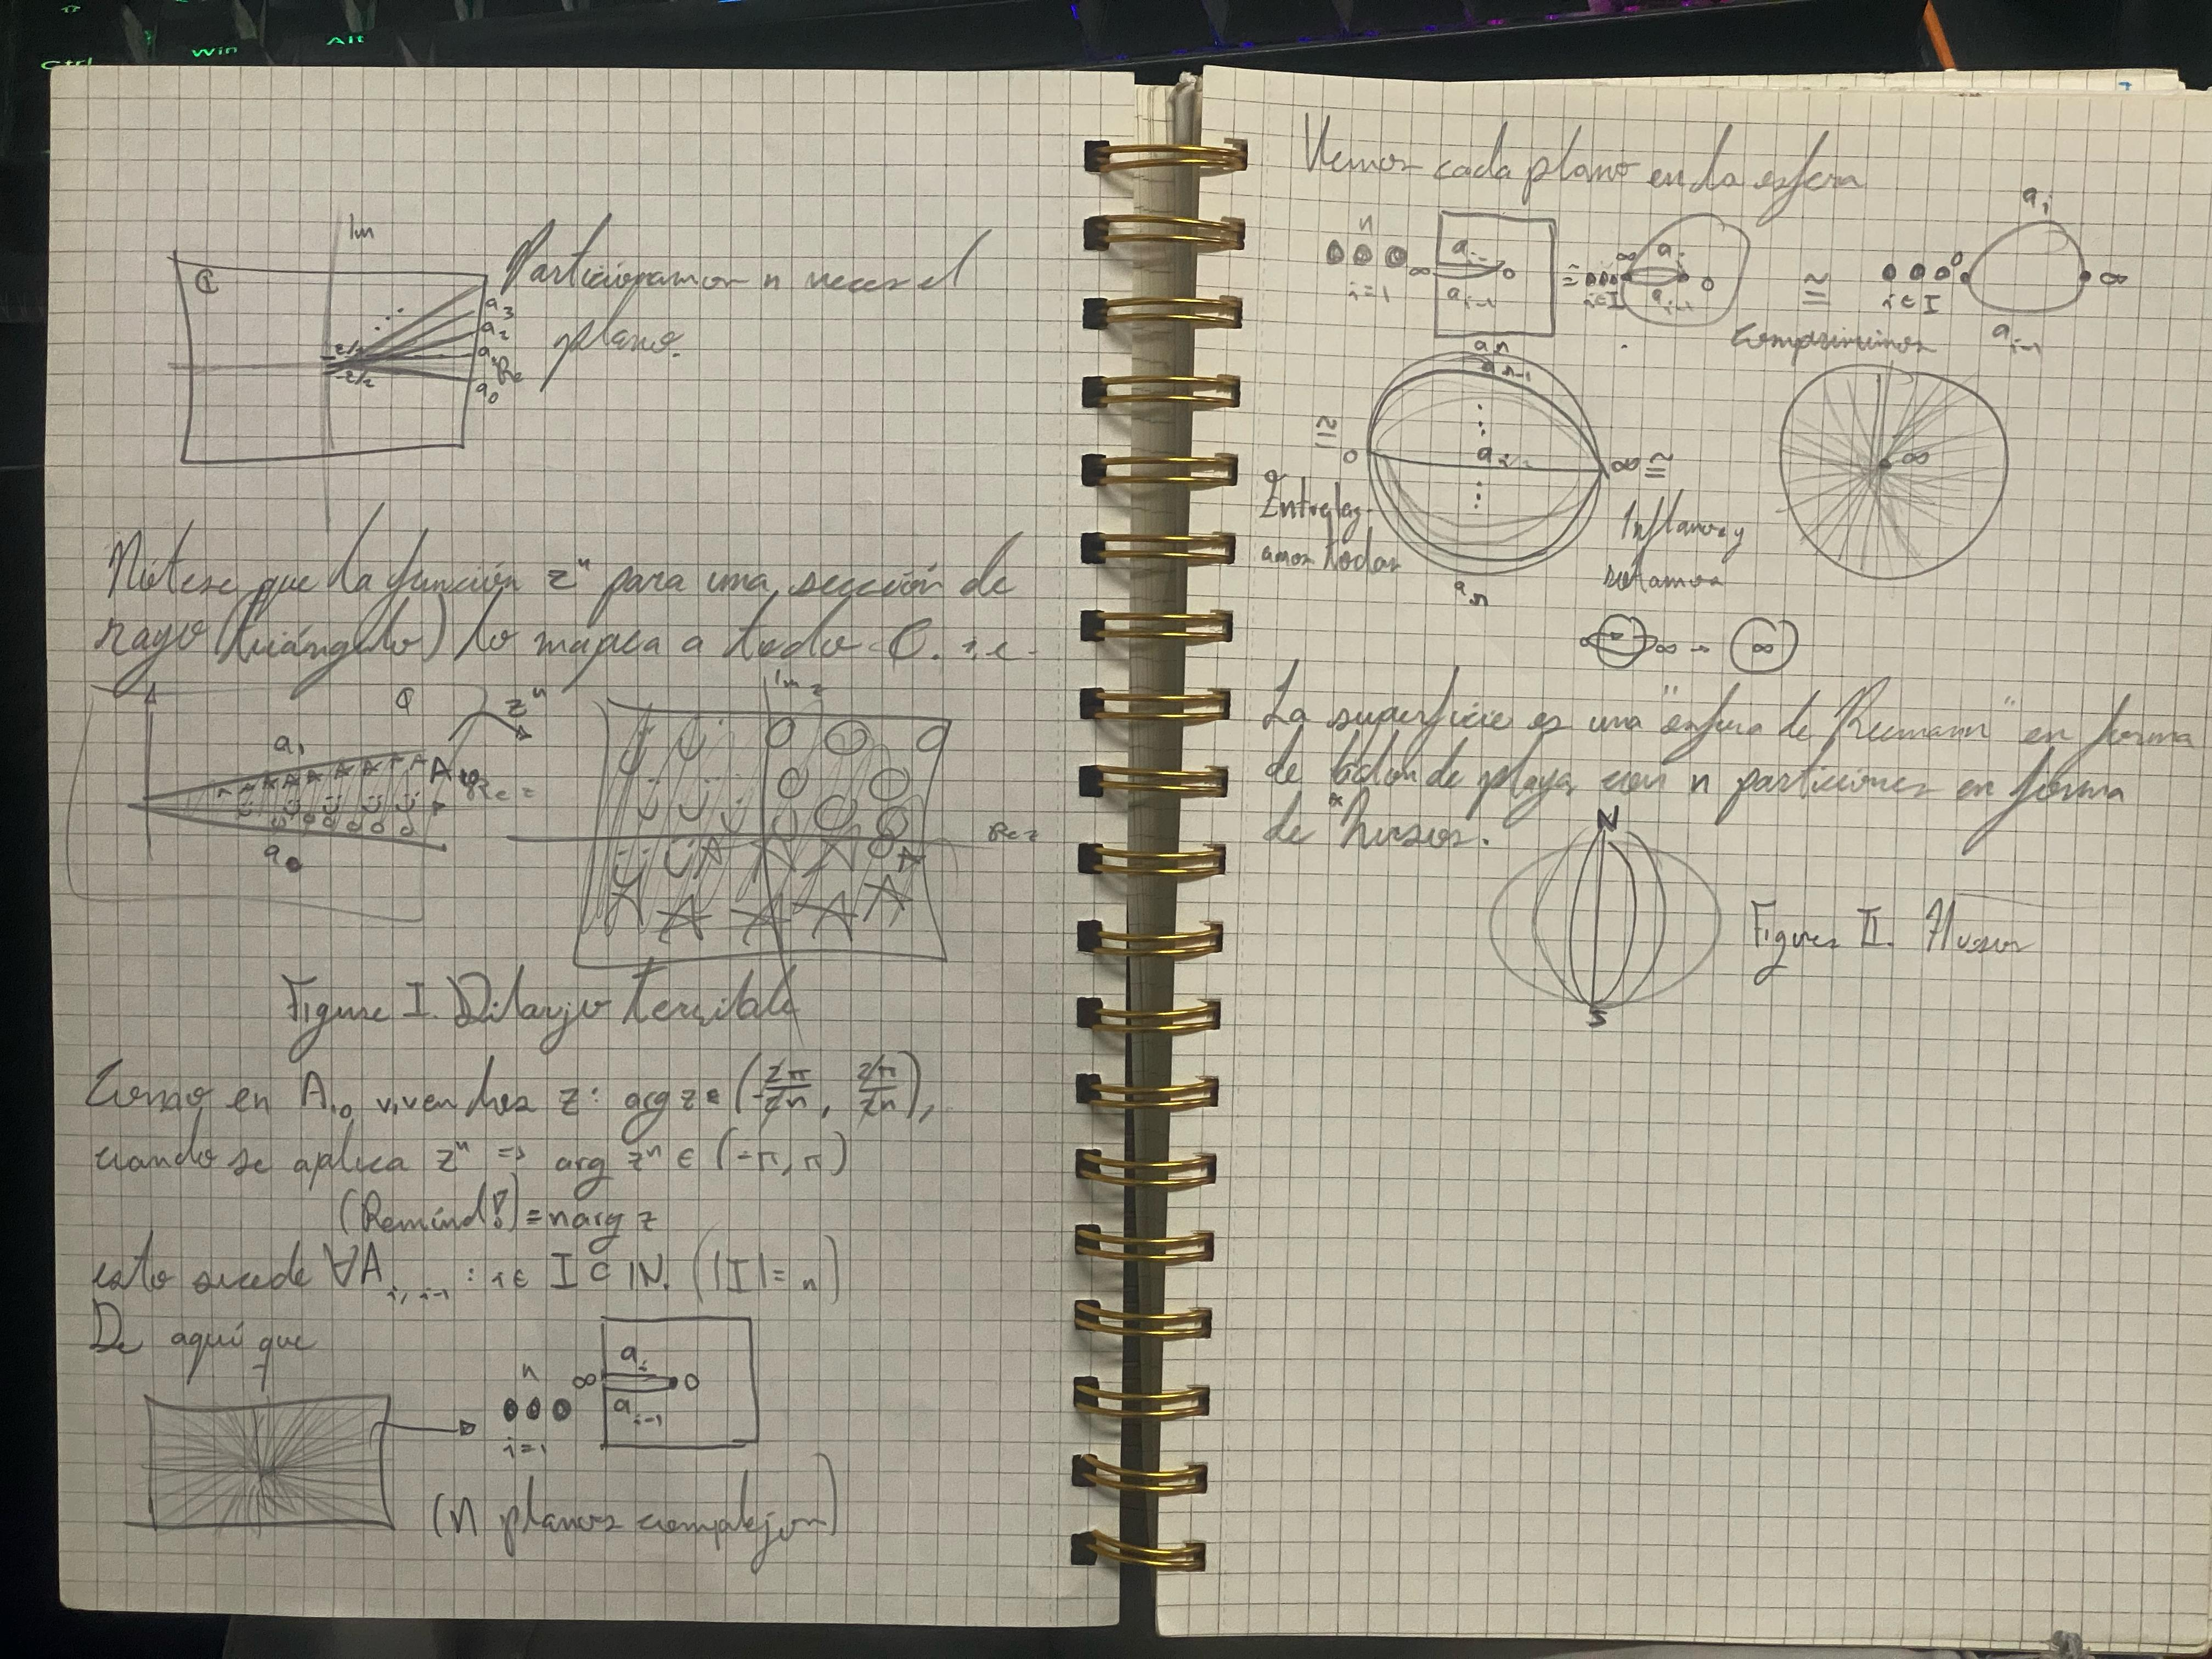
\includegraphics[width=1\linewidth]{ej1.jpg}
    \caption{*Versión visual del ej. 1 parte 1}
    \label{fig:enter-label}
\end{figure}

\end{document}
